\documentclass[4paper]{article}
\usepackage[spanish]{babel}
%\usepackage[ansinew]{inputenc}
\usepackage[utf8x]{inputenc}
%\usepackage[utf-8]{inputenc}
%\usepackage[T1]{fontenc}
\usepackage{graphicx}
\usepackage{multicol}
\usepackage{longtable}
\usepackage{array}
\usepackage{multirow}

\renewcommand{\tablename}{Tabla}

\author{Examen tercera evaluación}
\title{Tipo B}
\date{\today}

\begin{document}
\maketitle 
%\tableofcontents
%\newpage
\vspace{2cm}
\begin{center}
\begin{large}
%\textbf{Diagrama UML de la aplicación}
\end{large}
\end{center}\par 
%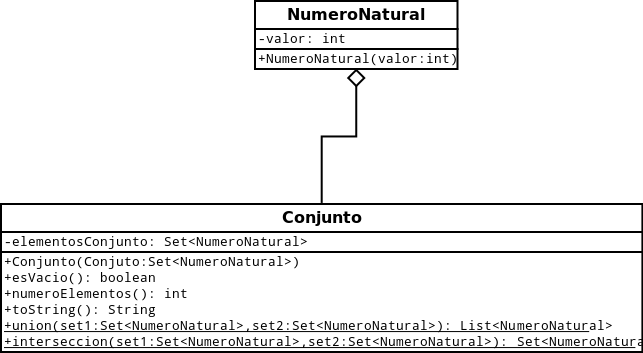
\includegraphics[scale=0.45]{UML.png}
\vspace{0.5cm}
\section*{Ejercicio 1}
Queremos realizar un programa para la gestión de equipos de futbol. Un equipo de futbos consta de una plantilla formada por 11 jugadores mas un entrenador y su ayudante.\par
De todos ellos necesitamos saber su nombre y DNI. Para el caso de los  jugadores debemos saber de todos el número de años jugando en primera división.\\
Para el caso de los 2 delanteros también debemos conocer el número de goles marcados en la última temporada. Por otra parte para los 4 centrocampista debemos saber el número de pases acertados la última temporada. Para los defensas nos interesa conocer el número de pases interceptados la pasada temporada y para el caso del portero solicitaremos el número de goles encajados.\par 
Para el entrenador y ayudante necesitamos saber los años de experiencia, y en el caso el nombre del entrenador el número de años que lleva en primera división y para el ayudante el último entrenador a que acompañó.

\begin{itemize}
\item Debes crear un equipo de 11 jugadores y el entrenador y ayudante. Para esto crea una clase denominda \emph{EquipoFutbol} y que tenga como atributo propio la fecha de creación que será el momento en que se crea una instancia de dicha clase.
\item Crea dos colecciones, que sean atributos de instancia, denominadas \emph{cuerpoTecnico} y \emph{jugadores}.
\item En el constructor de esta clase debes pasar como parámetro un objeto \emph{File} que es el descriptor que apunta al fichero con los datos de los componentes del equipo denominado equipo.csv. Dichos datos sirven para rellenar las dos listas anteriores.
\item Crea un archivo denominado \emph{TestEquipo} que cree una instancia de \emph{EquipoFutbol}.
\item Muestra por pantalla las dos listas que crea el equipo
\item Vuelca estas dos colecciones en un fichero de texto, denominado \emph{outEquipo.txt}
\item Crea una excepción propia denominada \emph{MourinhoExcepcion} que se lance cuando se intente crear un entrenador cuyo atributo nombre sea \emph{Mouriño}
\item Crea el correspondiente diagrama UML.
\end{itemize}

\section*{Criterios de evaluacion}
Los criterios de evaluación son los indicados a continuación:\par 
\vspace*{0.5cm}
\begin{tabular}{|c|c|}
\hline
\textbf{CRITERIO EVALUACION} & \textbf{PUNTUACION} \\
\hline
Relaciones de herencia bien & 1.5 pto.\\
\hline
Fichero java de herencia bien & 2 ptos. \\
\hline
Excepción propia funcionando correctamente & 1 pto.\\
\hline
Lectura de los datos con Scanner & 2 ptos.\\
\hline 
Diagrama UML & 1 pto.\\
\hline
Archivo TestEquipo & 1 pto.\\
\hline
Escritura de datos en archivo outEquipo.txt & 1.5 ptos.\\
\hline
\end{tabular}
\\
\\
En el caso de que no seas capaz de leer los datos para crear los objetos correspondientes del fichero \emph{equipo.csv} e incluirlos en las listas, puedes crearlo manualmente para posteriormente volcarlos al fichero \emph{outEquipo.txt} y pueda ser valorado. Lógicamente no se valorará la parte de lectura del fichero y parte de la lógica del fichero Test.
\section*{Subida de ficheros}
Comprime el directorio de trabajo de eclipse. Debes incluir el diagrama UML, bien en el propio directorio del proyecto o bien aparte. 
\end{document}
